\documentclass[11pt]{article}
\usepackage[margin=1in]{geometry}
\usepackage{amsmath,amssymb,booktabs,enumitem,hyperref,array,graphicx}
\usepackage[T1]{fontenc}
\usepackage{lmodern}
\hypersetup{colorlinks=true,urlcolor=blue,linkcolor=blue}
\setlist{nosep}
\emergencystretch=3em

\title{FRE-GY 9743 --- Assignment 7\\ \large A Monotone Convex Interpolator for Instantaneous Forward Rates}
\author{Yuri Moghaddam}
\date{November 2026}

\begin{document}
\maketitle

\noindent\textbf{Repository:}\\
{\small\url{https://github.com/Yuri48/FRE-GY-9743-Assignments-7/tree/Yuri_Moghaddam_Branch}}

\noindent\textbf{Code:} \texttt{Interpolator1DMonotoneConvex} in \texttt{fixedincomelib/utilities/numerics.py}.\\
\textbf{Notebook:} \texttt{hw7\_monotone\_convex\_interpolator.ipynb}. It runs end to end: it plots the IFR curves, prices the three products under both interpolators, and its last section checks the interpolator and all six PVs independently (fine-grid shape tests, Gauss--Legendre quadrature of the curve, discount-factor-only product formulas).

\section*{1. The problem}

The state data of each curve are IFR point values $f_i$ at node times $t_0<\dots<t_n$ (ACT/ACT years from the value date), and discount factors are $P(T)=\exp\bigl(-\int_0^T f(t)\,dt\bigr)$. The interpolant must be continuous, pass through every $(t_i,f_i)$ and, for compatible data, be monotone and convex between the nodes, with FLAT extrapolation outside $[t_0,t_n]$. Hagan and West's monotone convex method solves a related problem: there the inputs are \emph{discrete} forwards (interval averages) and the node values are derived from them. Here the node values are given, so I keep Hagan and West's structure (a quadratic per interval, with one extra breakpoint where needed) and choose the shape inside each interval instead of the node values.

\section*{2. Construction}

Write $h_i=t_i-t_{i-1}$ and $d_i=(f_i-f_{i-1})/h_i$ for the secant of interval $i$.

\paragraph{Step 1: node slopes.} At an interior node,
\[
s_i=\begin{cases}
\operatorname{sign}(d_i)\,\min\Bigl(\Bigl|\dfrac{h_{i+1}d_i+h_i d_{i+1}}{h_i+h_{i+1}}\Bigr|,\;2\min(|d_i|,|d_{i+1}|)\Bigr) & d_i d_{i+1}>0,\\[2mm]
0 & d_i d_{i+1}\le 0 \ \text{(local extremum)},
\end{cases}
\]
the three-point (parabolic) slope, capped. At the ends, $s_0=2d_1-s_1$ and $s_n=2d_n-s_{n-1}$, which makes each end interval a single quadratic. Every $s_i$ lies between its two neighbouring secants and has their sign (or is zero), and the cap gives $|s_{i-1}|,|s_i|\le 2|d_i|$ on every interval.

\paragraph{Step 2: one knot per interval.} By the mean value theorem, any $C^1$ interpolant has slope $d_i$ somewhere in $(t_{i-1},t_i)$. I put a knot there,
\[
\xi_i=t_{i-1}+h_i\,\frac{s_i-d_i}{s_i-s_{i-1}},
\]
and let the slope be linear on each side: $s_{i-1}\to d_i$ on $[t_{i-1},\xi_i]$ and $d_i\to s_i$ on $[\xi_i,t_i]$. Each side is a quadratic; the two meet at $\xi_i$ with equal value and slope, and their rises add up to $h_i d_i$, so the curve lands exactly on $f_i$. In general, with $\alpha=\xi_i-t_{i-1}$ and $\beta=t_i-\xi_i$, the slope at the knot is $\bar s=(2h_i d_i-\alpha s_{i-1}-\beta s_i)/h_i$, which equals $d_i$ for this choice of $\xi_i$. If $s_{i-1}+s_i=2d_i$ the knot falls at the midpoint and the interval is a single quadratic. A quadratic $f$ is reproduced exactly, since its three-point slopes are exact.

\paragraph{Integration.} Each piece integrates to a cubic, so \texttt{integrate} is the difference of an exact antiderivative: cumulative integrals at the nodes are stored, and the FLAT regions add $f_0(t_0-a)$ and $f_n(b-t_n)$. Discount factors carry no quadrature error. One node gives the constant curve (the 5\,bp funding spread); two nodes give a straight line.

\section*{3. Why the curve is monotone and convex}

\paragraph{Claim.} If the nodes are increasing with strictly increasing secants, $0<d_1<d_2<\dots<d_n$, the curve is continuous, $C^1$, increasing and convex on $[t_0,t_n]$.

\paragraph{Proof.} An interior slope lies strictly between its secants, so $d_i<s_i<d_{i+1}$. At the ends, $s_0=2d_1-s_1<d_1$ and $s_0\ge 0$ because $s_1\le 2d_1$; symmetrically $s_n>d_n$. Hence $0\le s_{i-1}<d_i<s_i$ on every interval. The derivative rises linearly from $s_{i-1}$ to $d_i$ to $s_i$, so it is non-decreasing (convex) and non-negative (increasing) on each interval, and the curve stays between $f_{i-1}$ and $f_i$. The slopes agree at the nodes, so the derivative is continuous and non-decreasing on the whole of $[t_0,t_n]$: the curve is convex and increasing on the full node range, not just interval by interval. Decreasing data with secants rising towards zero is the mirror case. \hfill$\square$

The supplied secants are $20,27,39,50,60$\,bp/yr for SOFR and $14,20,26,40,50$\,bp/yr for Fed Funds, so both curves satisfy the claim. Figure~\ref{fig:curves} shows the curves and, on the right, the slope rising piecewise linearly and crossing each secant at the knot.

\begin{figure}[h]
\centering
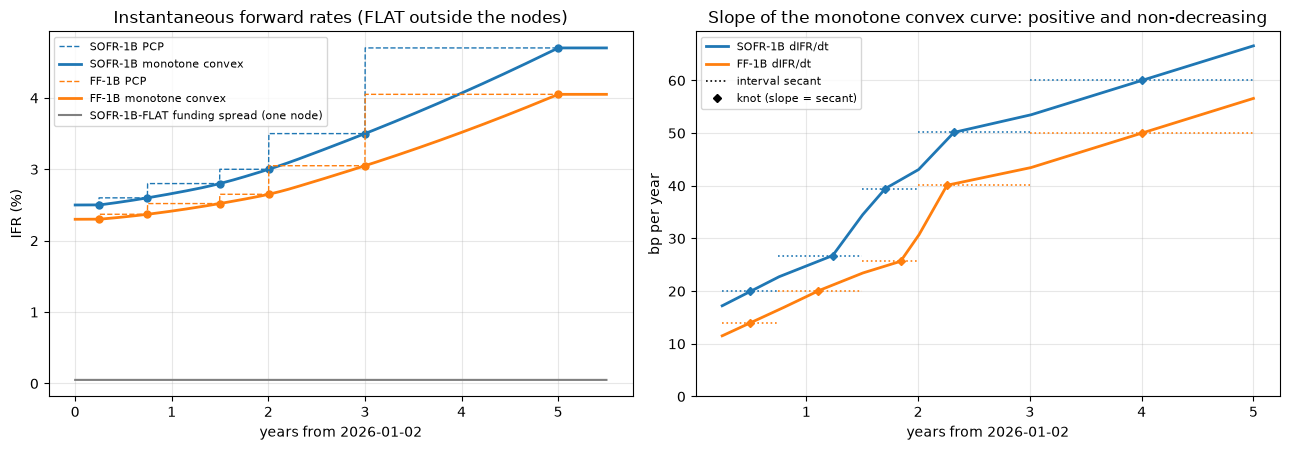
\includegraphics[width=\textwidth]{hw7_ifr_curves.png}
\caption{Left: IFR curves under PCP (dashed) and the monotone convex interpolator (solid), with the constant one-node funding spread. Right: slope of the monotone convex curves, each interval's secant (dotted) and the knots (diamonds).}
\label{fig:curves}
\end{figure}

\section*{4. Data that cannot satisfy every condition}

Continuity and passing through the nodes are never given up, and every interval stays monotone, so the curve never overshoots the node values. What gives way depends on the data (Figure~\ref{fig:bad}):
\begin{itemize}[leftmargin=*]
\item \textbf{Local extremum.} The slope at a hump or trough is 0. A trough is compatible with convexity (both sides stay convex). A $C^1$ curve cannot be convex on both sides of a peak, so the interval rising into a peak is concave: the curve bends the way the data bend.
\item \textbf{Secants that turn} (data convex at one end of an interval and concave at the other, $(s_{i-1}-d_i)(s_i-d_i)>0$). One inflection is unavoidable. The knot moves to the midpoint and holds it; the slope there is $2d_i-(s_{i-1}+s_i)/2$, which has the sign of $d_i$ because of the cap, so the interval is still monotone.
\item \textbf{Collinear nodes} ($d_i=d_{i+1}$). A convex curve through three collinear points is straight between them, so the interval is linear and the knot sits on the end node of the run, leaving a convex kink there. $C^1$ is what gives way, not monotonicity or convexity.
\item \textbf{Extrapolation.} FLAT extrapolation meets the curve with a kink at $t_0$ and $t_n$; a rising convex curve cannot flatten out at $t_n$ and stay convex.
\end{itemize}

\begin{figure}[h]
\centering
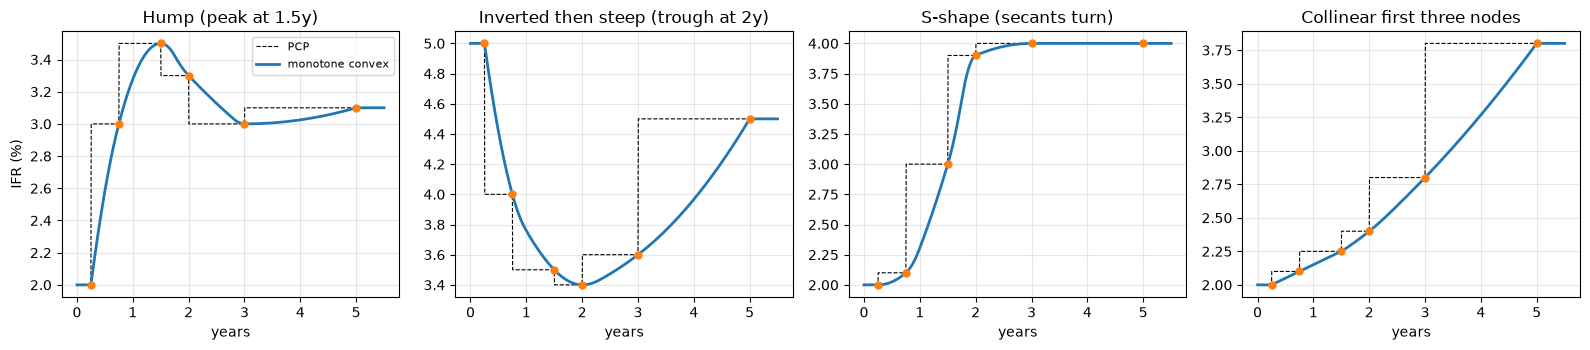
\includegraphics[width=\textwidth]{hw7_incompatible_data.png}
\caption{Incompatible data: monotone convex interpolator (solid) against PCP (dashed). Every interval is monotone and within its node values.}
\label{fig:bad}
\end{figure}

\section*{5. PV comparison}

\begin{center}
\small
\begin{tabular}{@{}lrrrcc@{}}
\toprule
 & & & & avg SOFR IFR & avg SOFR--FF \\
Product & PCP PV & MC PV & MC $-$ PCP & PCP / MC (\%) & PCP / MC (bp) \\
\midrule
FRA, receive 3.2\% & 2,908.29 & 3,261.72 & $+353.43$ & 2.637 / 2.567 & 23.9 / 22.0 \\
RFR swap, receive 3.4\% & 6,222.52 & 12,844.06 & $+6{,}621.54$ & 3.189 / 2.958 & 37.0 / 32.3 \\
Basis swap, receive SOFR+10\,bp & 8,351.35 & 7,623.30 & $-728.05$ & 2.999 / 2.834 & 33.4 / 29.5 \\
\bottomrule
\end{tabular}
\end{center}
Averages are over each product's start and end dates. Both curves are FLAT at the same values outside the nodes, so the differences come from inside the node range. The left-continuous step gives every interval $(t_{i-1},t_i]$ its right node's value $f_i$; for these upward-sloping curves that is the highest value on the interval, while the monotone convex curve stays between $f_{i-1}$ and $f_i$. So PCP projects higher forwards everywhere between the nodes and gives slightly lower discount factors.
\begin{itemize}[leftmargin=*]
\item \textbf{FRA.} The projected rate falls by about 7\,bp, worth $N\tau\times 7\,\text{bp}\times D_f\approx 10^6\times0.511\times0.0007\times0.98\approx 352$ to the fixed receiver.
\item \textbf{RFR swap.} The annual compounded SOFR coupons fall from 2.70 / 3.08 / 3.81\% to 2.60 / 2.90 / 3.37\%. The last coupon moves most because PCP applies the 5-year node (4.7\%) as soon as the curve passes 3 years, i.e.\ over the swap's final quarter. The floating leg falls by 6,283 and the fixed leg gains 338 from higher discount factors; the par rate drops from 3.18\% to 2.95\%.
\item \textbf{Basis swap.} Only the SOFR--FF basis matters. The node bases widen with maturity (20, 23, 28, 35, 45, 65\,bp); PCP uses each interval's right-node basis, the monotone convex basis moves gradually between nodes, so the average basis falls by about 4\,bp. Both legs lose value (SOFR $-3{,}057$, Fed Funds $-2{,}329$), and receiving SOFR loses 728 net.
\end{itemize}

\section*{6. Validation (notebook section 8)}
On both supplied curves the interpolant hits every node exactly, has equal one-sided slopes at the interior nodes, and is increasing and convex on a 20,001-point grid over $[t_0,t_n]$; \texttt{integrate} matches composite Gauss--Legendre quadrature of \texttt{interpolate} to $10^{-12}$ relative and is additive and antisymmetric; a quadratic is reproduced to machine precision. All six engine PVs match a re-pricing from quadrature-built discount factors and the closed forms (FRA $N\tau(K-F)D_f$, fixed leg $NK\sum\alpha_iD_f$, overnight leg $N\sum[(P^s_i/P^e_i-1)+\alpha_i s]D_f$) to within $5\times10^{-9}$.

\end{document}
